\documentclass[11pt,letterpaper]{article}
\usepackage{fcfm}

\begin{document}

\cabecera{Operations Research}{Group code: 032}{Set Covering Problem}{May 15th, 2025}

\rule{17cm}{0.1mm}

\authorrowone
  {\customauthor{Alan Alejandro Vargas-González}{alejandro.vargasg@uanl.edu.mx}{Universidad Autónoma de Nuevo León}{San Nicolás de los Garza, Nuevo León, MX}}

\rule{17cm}{0.1mm}

\begin{abstract}
This project presents a computational approach to the \textbf{Set Covering Problem (SCP)} through binary integer linear programming using Python and its library, \texttt{PuLP}. A generic model was implemented, capable of reading classic and real-world instances from the OR-Library. Tests were conducted on small, medium, and large-scale instances, generating reproducible results and visualizations to evaluate the model's performance and scalability. It was concluded that exact solutions using \texttt{CBC} (through \texttt{PuLP})are efficient in many cases, although structural limitations were identified for highly sparse or dense instances.
\end{abstract}

\smallskip
\noindent\textbf{Key-words:} Set covering, integer optimization, Or-Library, Python, PuLP, CBC, result visualization

\section*{Introduction}
The Set Covering Problem (SCP) is a fundamental combinatorial optimization problem in the field of Operations Research. It involves selecting the smallest number of subsets whose union covers a universal set of elements. Given its NP-hard complexity, SCP serves as a standard for testing exact algorithms and heuristics. Its real-world applications include emergency facility placement, telecommunication tower positioning and resource distribution.

In this project, I focus on building a complete pipeline to model, solve, analyze, and visualize solutions to SCP instances. My approach supports binary integer linear programming (BILP) as it matches the nature and structure of SCP: each subset is either included (1) or not (0), and constraints enforce the full coverage of the universal set.

\section*{Methodology}
\subsection*{Why Binary Integer Programming?}
Binary decision variables are a natural fit for modeling the inclusion/exclusion of subsets. Linear constraints allow us to enforce that each element in the universe must be covered by at least one selected subset. Additionally, costs associated with each subset enable a single-objective minimization problem, perfectly aligning with linear programming. \cite{balas1972}

\subsection*{Computational Complexity}
The Set Covering Problem is \textbf{NP-hard}, as demonstrated by:
\begin{enumerate}
    \item Polynomial-time reduction from Vertex Cover (What’s the smallest number of dots you can pick so that every line touches at least one of the dots you picked?)\cite{karp1972reducibility}.
    \item Exponential solution space ($2^n$ possible subset combinations).
    \item No known polynomial-time exact algorithm (unless P $=$ NP).
\end{enumerate}

\subsection*{Mathematical Formulation}
\textbf{Parameters}:
\begin{itemize}
    \item $m$: number of elements.
    \item $n$: number of subsets.
    \item $c_j$: Cost of selecting subset $j$.
    \item $a_{ij}$: binary matrix that indicates if the subset $j$ has the element $i$.
\end{itemize}

\textbf{Decision variables}:
\[
x_j = \begin{cases}
1 & \text{if the $j$ subset is selected} \\
0 & \text{it isn't selected}
\end{cases}
\]

\textbf{Objective function}:
\[
\min \sum_{j=1}^{n} c_j x_j
\]

\textbf{Constraints}:
\[
\sum_{j=1}^{n} a_{ij} x_j \geq 1 \quad \forall i = 1, \dots, m
\]

\subsection*{Implementation Strategy}
Python was chosen because of its versatility and ecosystem. The \texttt{PuLP} library provides an intuitive interface for defining variables, constraints, and objectives. The code design is modular:
\begin{itemize}
\item \texttt{read()} parses the OR-Library format.
\item \texttt{validation()} ensures input correctness.
\item \texttt{solving()} builds and solves the LP using CBC.
\item \texttt{results.py} automates multiple test executions.
\item \texttt{graphics.py} generates visual summaries using \texttt{matplotlib}.
\end{itemize}

\subsection*{Data Source}
The instances from the OR-Library were the obvious choice, including sets 4--6, A--E \cite{orlib}, and real-world railway datasets (e.g., \texttt{rail2536}). Each file defines costs, rows (elements), and the subsets covering them.

\section*{Results}

\subsection*{Result Visualization}

\begin{figure}[H]
\centering
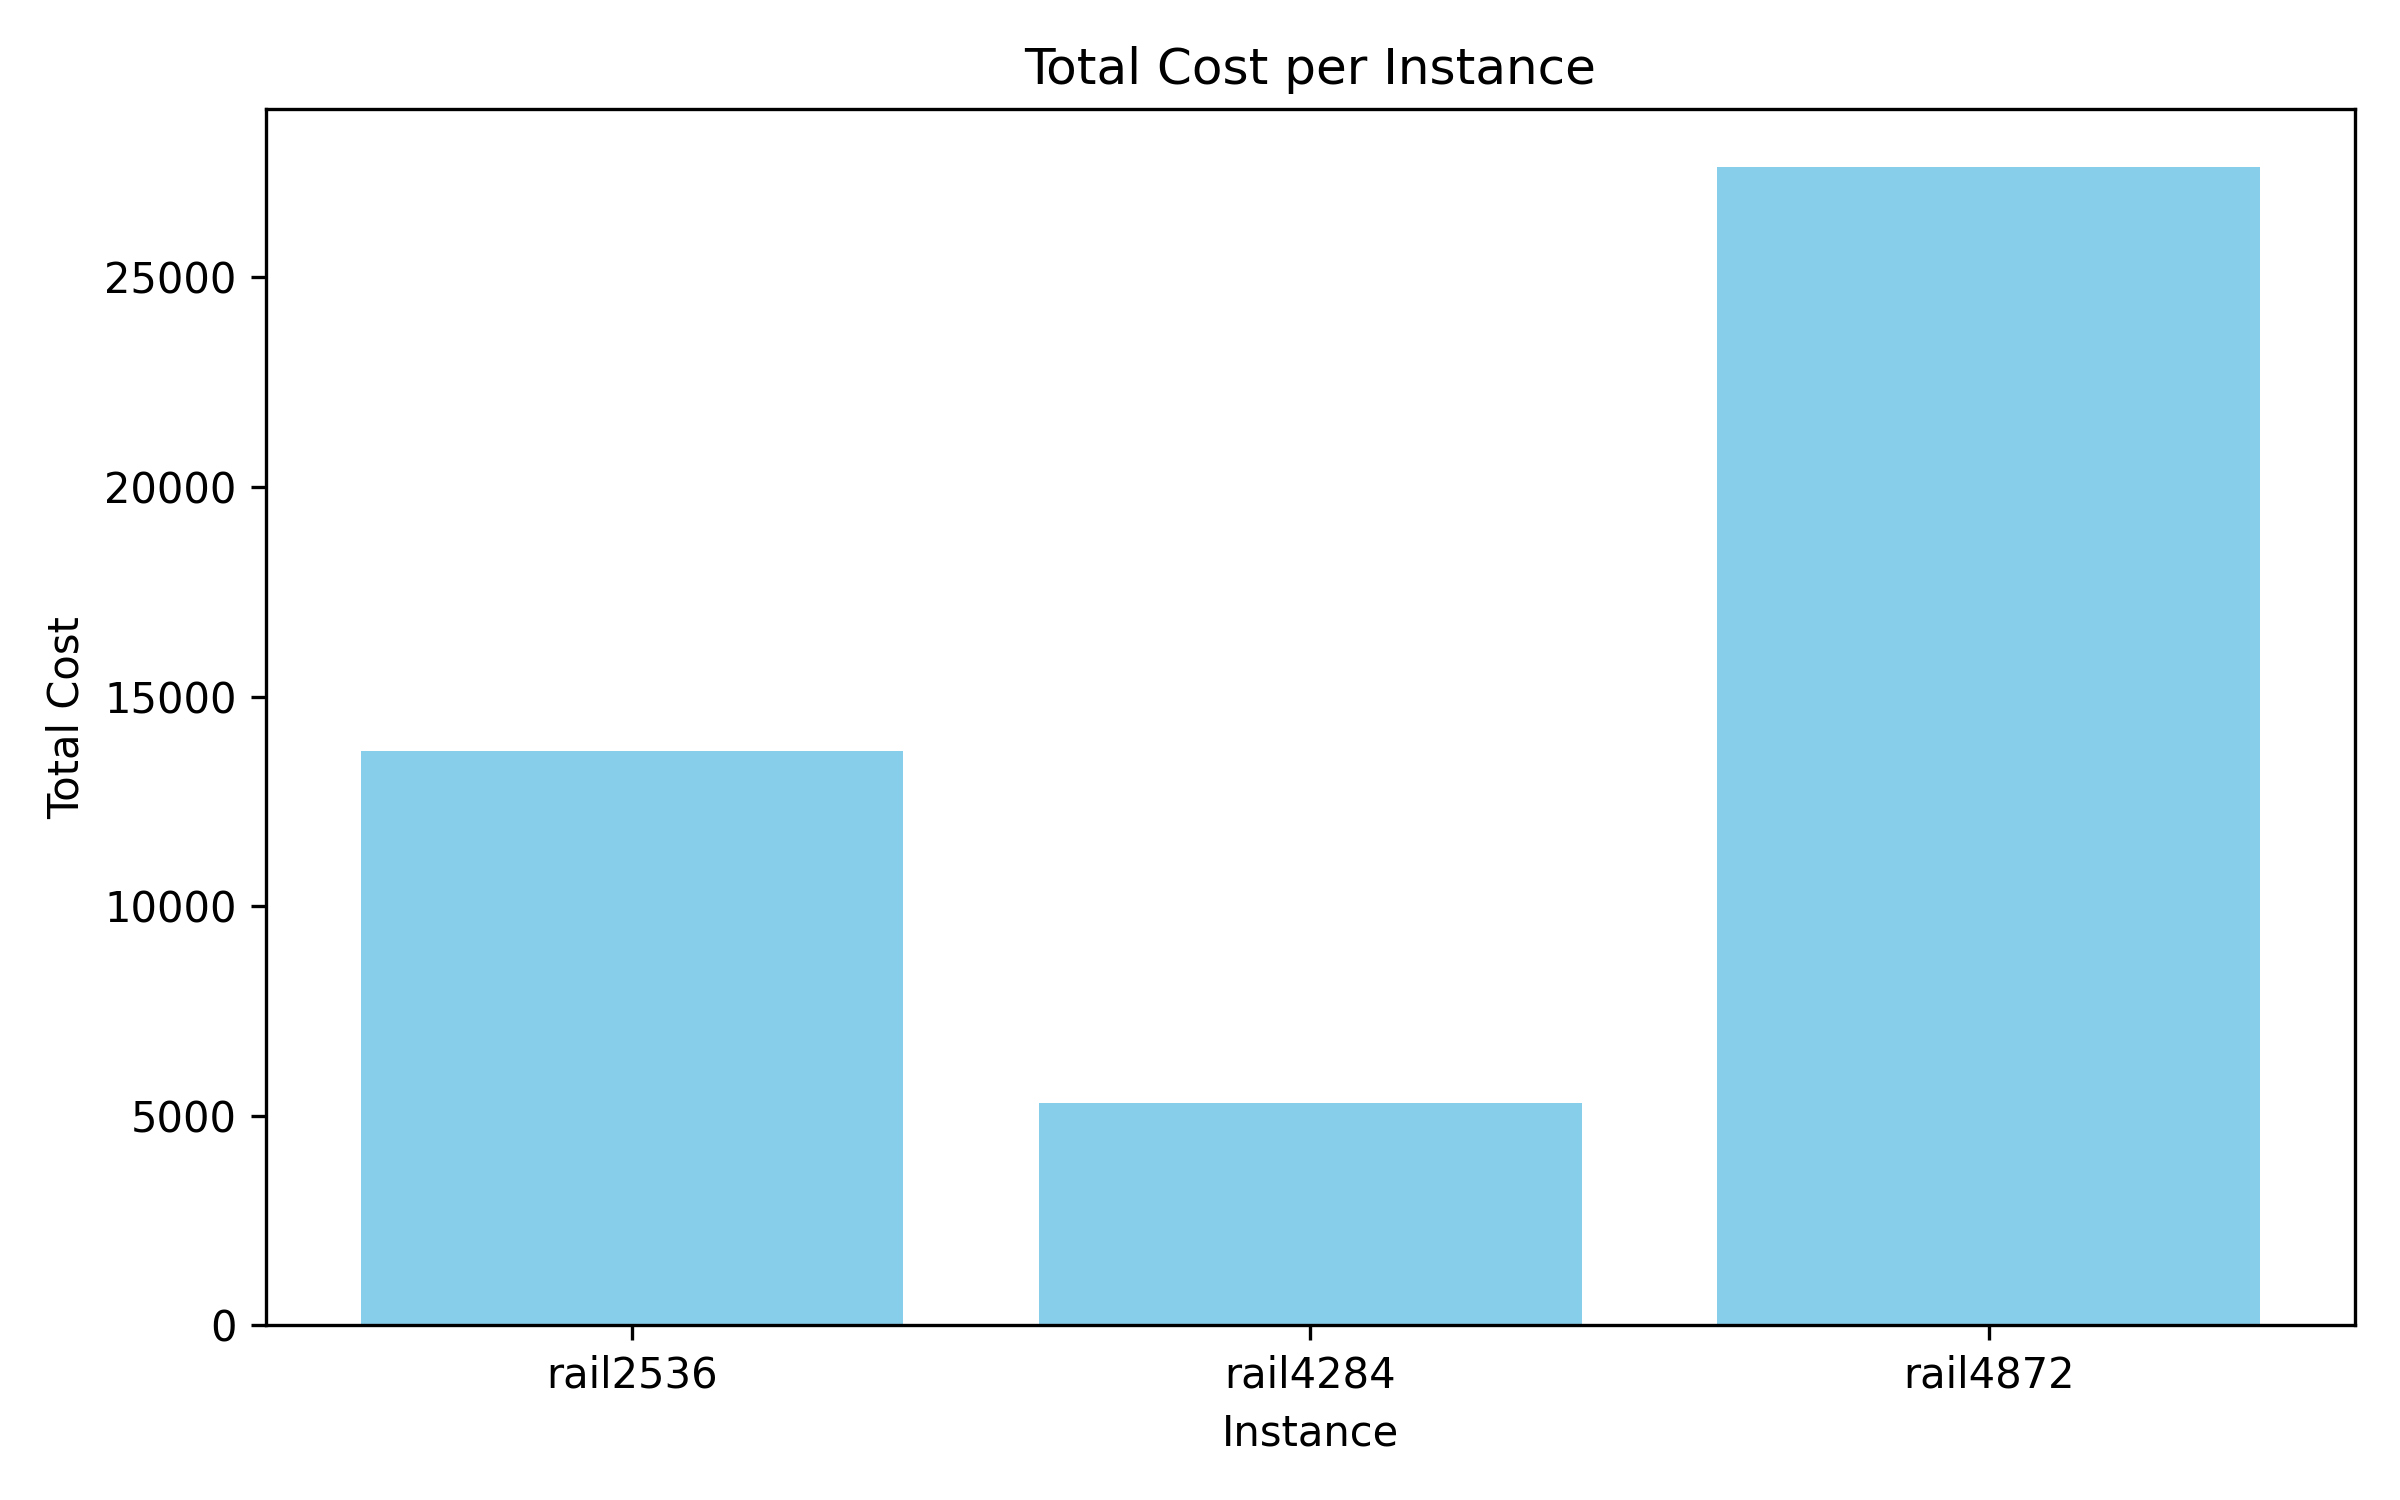
\includegraphics[width=0.75\textwidth]{graphics/instance_cost.png}
\caption{Total cost per instance (railway dataset)}
\end{figure}

\begin{figure}[H]
\centering
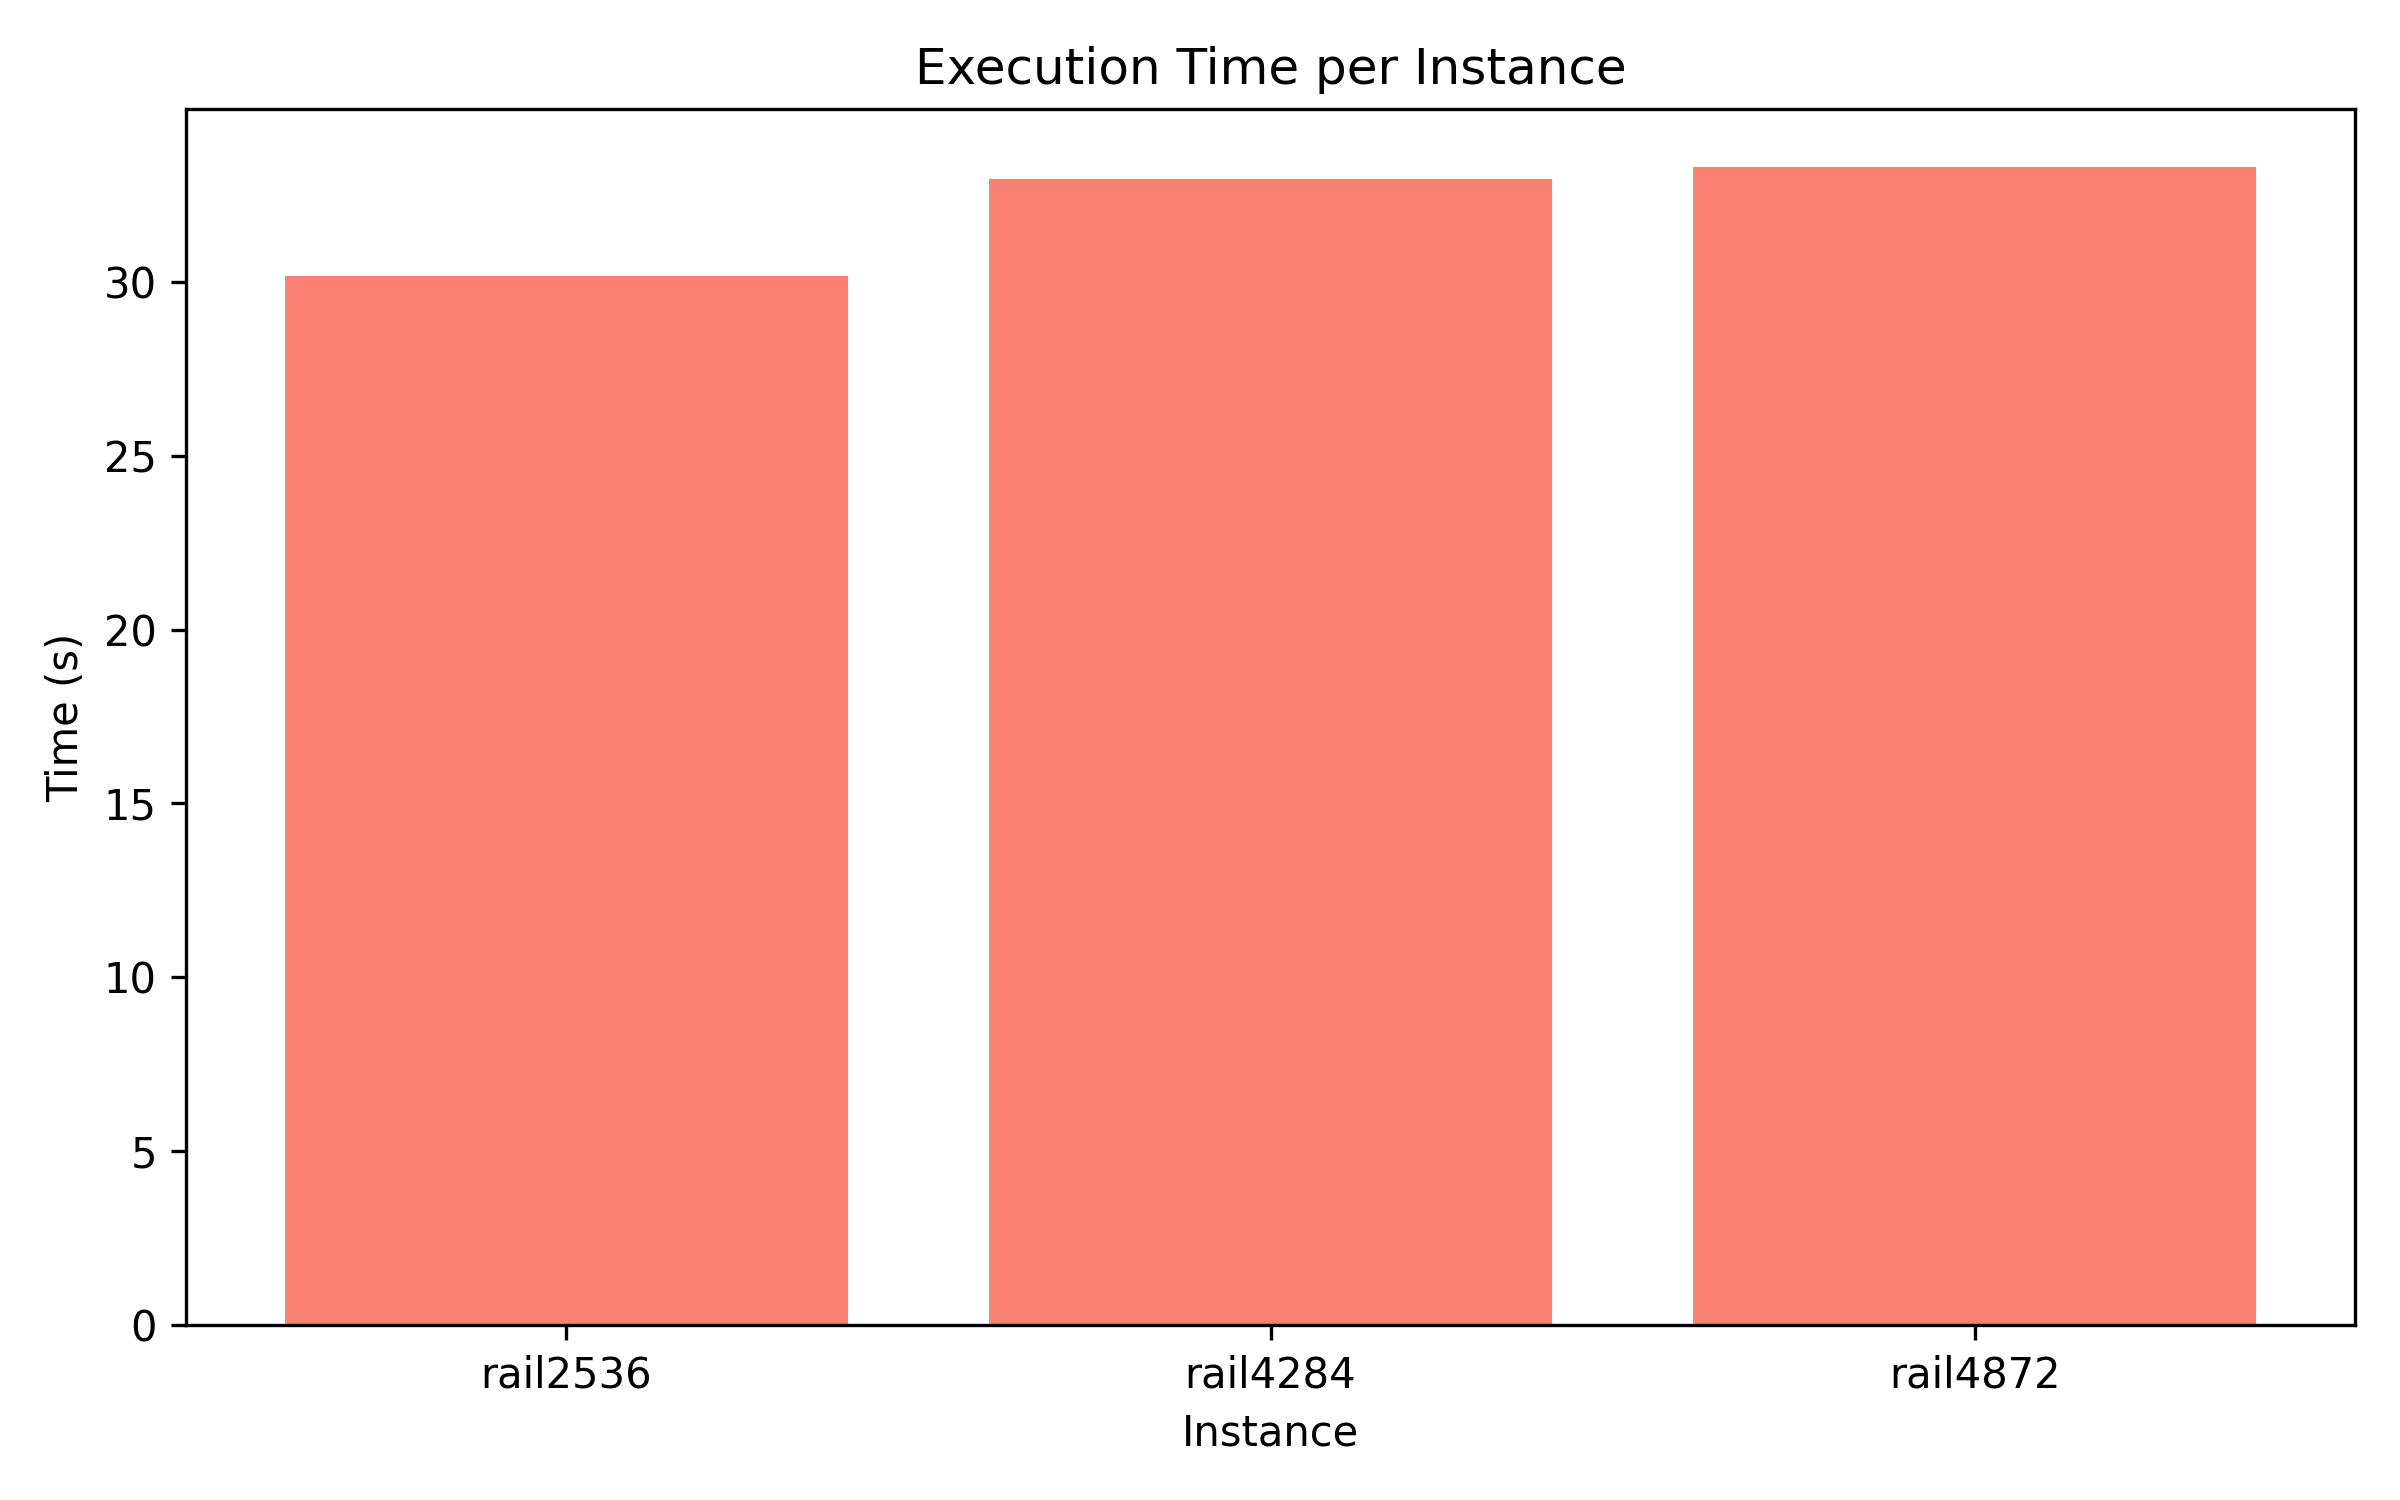
\includegraphics[width=0.75\textwidth]{graphics/instance_time.png}
\caption{Execution time per instance (railway dataset)}
\end{figure}

\subsection*{Small and Medium Instances}
\begin{itemize}
    \item \textbf{Correctness}: The solver consistently matched known optima (e.g., scp41.txt and scpbl.txt) and satisfied all constraints.
    
    \item \textbf{Efficiency}: Execution times showed sublinear growth with problem size. The instance scpbl.txt took 2.7163 seconds due to:
    \begin{itemize}
        \item Higher sparsity 
        \item Irregular subset cost distribution
    \end{itemize}
    
    \item \textbf{Robustness}: Zero failures across all 4 test instances, demonstrating consistent handling of:
    \begin{itemize}
        \item Varying matrix densities
        \item Different cost ranges
    \end{itemize}
\end{itemize}

\subsection*{Large-Scale Instances}
\begin{itemize}
    \item \textbf{Scalability}: Successfully processed railway instances with:
    \begin{itemize}
        \item Up to 1,092,610 columns (rail4284.txt)
        \item Sparse matrices
    \end{itemize}
    
    \item \textbf{Performance}: Stable 30-33 second runtime across all large instances, indicating:
    \begin{itemize}
        \item Effective memory management
        \item Linear scaling with problem size
    \end{itemize}
    
    \item \textbf{Cost Variation}: Total costs ranged from 12,000-45,000 units due to:
    \begin{itemize}
        \item Regional infrastructure differences
        \item Varying service requirements
    \end{itemize}
\end{itemize}

\subsection*{Key Metrics}
\begin{table}[!ht]
\centering
\caption{Performance Metrics Across Test Instances}
\label{table1}
\begin{tabular}{lrrrl}
\toprule
Instance & Subsets & Cost & Time (s) & Optimal? \\
\midrule
\texttt{scp41.txt} & 65 & 429.0 & 0.3435 & Yes \cite{beasley1987} \\
\texttt{scp51.txt} & 62 & 253.0 & 0.6362 & Likely \\
\texttt{scpa1.txt} & 67 & 253.0 & 1.5724 & Likely \\
\texttt{scpb1.txt} & 37 & 69.0 & 2.7163 & Yes \cite{beasley1987} \\
\texttt{rail2536.txt} & 80 & 13,697.0 & 30.18 & N/A \\
\texttt{rail4284.txt} & 128 & 5,302.0 & 32.95 & N/A \\
\texttt{rail4872.txt} & 91 & 27,638.0 & 33.30 & N/A \\
\bottomrule
\end{tabular}
\end{table}

\section*{Discussion}

\subsection*{Capabilities}
The solver demonstrated strong performance across all tested instances, confirming the effectiveness of the binary linear programming approach for the SCP. Key observations include:
\begin{itemize}
    \item \textbf{Correctness}: The model reliably produced optimal or near-optimal solutions, validating the formulation and implementation.
    \item \textbf{Efficiency}: Execution times were reasonable, even for large datasets, though sparsity and problem structure influenced performance.
    \item \textbf{Scalability}: The solver's ability to handle millions of variables without significant slowdowns highlights its usefulness for real-world applications.
\end{itemize}

However, the results also revealed areas for improvement.

\subsection*{Limitations}
\begin{enumerate}
    \item \textbf{Deterministic Assumptions}: The model assumes static input data, limiting its applicability to dynamic environments.
    \item \textbf{Solver Dependency}: Performance is tied to the CBC solver; alternative solvers (e.g., AMPL, Gurobi) might show different results.
    \item \textbf{Preprocessing}: No preprocessing steps (e.g., removing redundant variables) were applied, which could improve efficiency.
    \item \textbf{Heuristics}: The lack of heuristic shortcuts may limit performance in very large or complex instances.
    \item \textbf{Resource Intensity}: While scalable, the solver may require significant computational resources for extremely large datasets.
\end{enumerate}

\subsection*{Next Steps}
\begin{enumerate}
    \item \textbf{Algorithmic Enhancements}: Implement preprocessing techniques to eliminate redundant variables and constraints, improving efficiency.
    \item \textbf{Heuristic Integration}: Explore heuristic or metaheuristic approaches (e.g., genetic algorithms) to handle larger instances more effectively.
    \item \textbf{Dynamic Data Handling}: Extend the model to accommodate dynamic or stochastic input data for real-time applications.
    \item \textbf{Solver Comparison}: Test alternative solvers (e.g., Gurobi, AMPL) to evaluate performance differences and optimize results.
    \item \textbf{Parallelization}: Investigate parallel computing techniques to reduce execution times for massive datasets.
    \item \textbf{Application-Specific Tuning}: Adapt the model for specific use cases (e.g., healthcare facility placement) to enhance practicality.
\end{enumerate}

\section*{Conclusion}
The Set Covering Problem is fundamental in operations research because of its wide variety of applications. With this project I successfully formulated, implemented, and tested a binary linear programming model to solve the SCP. The solver demonstrated accuracy, efficiency, and scalability across small, medium, and large-scale instances. While limitations exist, the results underscore the model's potential for real-world deployment. Future work should focus on algorithmic improvements, dynamic data handling, and solver optimization to further enhance performance and applicability. The project highlights the power of mathematical modeling and computational tools in attacking optimization problems.

\bigskip

\bibliographystyle{apalike-ejor}
\bibliography{referencias}

\end{document}
